\documentclass[10pt,a4paper]{article}

% ============================================================================
% KORA — paramètres éditables du dossier SAFINUM
% Modifiez uniquement les valeurs ci-dessous pour personnaliser le livrable.
% ============================================================================

\newcommand{\PrototypeName}{KORA}
\newcommand{\TeamName}{KORA TEAM}
\newcommand{\ChallengeName}{SAFINUM Innovate Challenge 2026}
\newcommand{\DocumentDate}{14 novembre 2026}

% Liens publics à vérifier avant le dépôt du formulaire SAFINUM.
\newcommand{\RepoURL}{https://github.com/kaezerwatto/KORA}
\newcommand{\DemoVideoURL}{https://raw.githubusercontent.com/kaezerwatto/KORA/master/release/KORA_Demo_Pitch_SAFINUM_2026.mp4}
\newcommand{\ChallengeURL}{https://safinum.cm/hackathon-test}

% Coordonnées officielles de l’équipe.
\newcommand{\TeamLead}{AZAB A RANGA FRANCK MIGUEL}
\newcommand{\TeamLeadEmail}{miguel.azab@facsciences-uy1.cm}
\newcommand{\TeamLeadPhone}{+237 686 826 745}
\newcommand{\MemberTwo}{BELL AQIL}
\newcommand{\MemberTwoEmail}{aqil.bell@facsciences-uy1.cm}
\newcommand{\MemberThree}{SIMO SIGEU NKOUAMKAM MENELIK}
\newcommand{\MemberThreeEmail}{menelik.simo@facsciences-uy1.cm}
\newcommand{\LinguisticValidator}{M. JEAN-ERNEST SOUROUMBAI}


\usepackage{fontspec}
\usepackage[french]{babel}
\defaultfontfeatures{Ligatures=TeX}
\setmainfont[
  Path=assets/fonts/,
  Extension=.ttf,
  UprightFont=NotoSans-Regular,
  BoldFont=NotoSans-Bold,
  ItalicFont=NotoSans-Italic,
  BoldItalicFont=NotoSans-BoldItalic
]{Noto Sans}
\setsansfont[
  Path=assets/fonts/,
  Extension=.ttf,
  UprightFont=NotoSans-Regular,
  BoldFont=NotoSans-Bold,
  ItalicFont=NotoSans-Italic,
  BoldItalicFont=NotoSans-BoldItalic
]{Noto Sans}
\setmonofont[
  Path=assets/fonts/,
  Extension=.ttf,
  UprightFont=NotoSansMono-Regular
]{Noto Sans Mono}
\usepackage{microtype}
\usepackage{amsmath}
\usepackage{amssymb}
\usepackage[a4paper,top=20mm,bottom=21mm,left=20mm,right=20mm,headheight=16pt]{geometry}
\usepackage{graphicx}
\usepackage{array}
\usepackage{booktabs}
\usepackage{longtable}
\usepackage{tabularx}
\usepackage{multicol}
\usepackage{enumitem}
\usepackage{ragged2e}
\usepackage{caption}
\usepackage{float}
\usepackage{xcolor}
\usepackage{tikz}
\usetikzlibrary{arrows.meta,backgrounds,calc,fit,positioning,shapes.geometric}
\usepackage[most]{tcolorbox}
\usepackage{listings}
\usepackage{xurl}
\usepackage{hyperref}
\usepackage{fancyhdr}
\usepackage{titlesec}
\usepackage{lastpage}

\definecolor{Ink}{HTML}{101A24}
\definecolor{InkSoft}{HTML}{243442}
\definecolor{Teal}{HTML}{0E9F85}
\definecolor{TealDark}{HTML}{087663}
\definecolor{Mint}{HTML}{DDF4EF}
\definecolor{Gold}{HTML}{F1B93B}
\definecolor{Warm}{HTML}{F7F3EA}
\definecolor{Paper}{HTML}{FAFBFC}
\definecolor{Slate}{HTML}{5C6D78}
\definecolor{Line}{HTML}{D8E0E5}
\definecolor{Risk}{HTML}{B4463B}
\definecolor{Success}{HTML}{247A5A}

\hypersetup{
  colorlinks=true,
  linkcolor=TealDark,
  urlcolor=TealDark,
  citecolor=TealDark,
  pdfauthor={\TeamName},
  pdftitle={KORA — Dossier technique SAFINUM Innovate Challenge 2026},
  pdfsubject={Extension Chrome locale FR/EN vers fulfulde de l’Adamaoua},
  pdfkeywords={KORA, SAFINUM, Fulfulde, fub, finance, inclusion}
}

\setlength{\parindent}{0pt}
\setlength{\parskip}{4.5pt}
\setlist[itemize]{leftmargin=5mm,itemsep=2pt,topsep=3pt}
\setlist[enumerate]{leftmargin=6mm,itemsep=2pt,topsep=3pt}
\renewcommand{\arraystretch}{1.18}

\titleformat{\section}
  {\Large\bfseries\color{Ink}}
  {\colorbox{Teal}{\color{white}\strut\thesection}}
  {0.65em}{}
  [\vspace{-0.35em}{\color{Gold}\rule{\linewidth}{0.7pt}}]
\titleformat{\subsection}{\large\bfseries\color{InkSoft}}{\thesubsection}{0.55em}{}
\titleformat{\subsubsection}{\normalsize\bfseries\color{TealDark}}{\thesubsubsection}{0.5em}{}
\titlespacing*{\section}{0pt}{1.2em}{0.65em}
\titlespacing*{\subsection}{0pt}{0.9em}{0.35em}

\pagestyle{fancy}
\fancyhf{}
\fancyhead[L]{\small\color{Slate}\textbf{KORA} · Dossier technique}
\fancyhead[R]{\small\color{Slate}\ChallengeName}
\fancyfoot[L]{\small\color{Slate}\TeamName}
\fancyfoot[R]{\small\color{Slate}\thepage/\pageref{LastPage}}
\renewcommand{\headrulewidth}{0.3pt}
\renewcommand{\footrulewidth}{0pt}

\newcolumntype{Y}{>{\RaggedRight\arraybackslash}X}
\newcolumntype{L}[1]{>{\RaggedRight\arraybackslash}p{#1}}
\newcolumntype{C}[1]{>{\Centering\arraybackslash}p{#1}}

\newtcolorbox{keybox}[1][]{
  enhanced,breakable,colback=Mint,colframe=Teal,
  boxrule=0.6pt,arc=2.5mm,left=3.2mm,right=3.2mm,top=2.6mm,bottom=2.6mm,
  fonttitle=\bfseries\color{Ink},title=#1
}
\newtcolorbox{warningbox}[1][]{
  enhanced,breakable,colback=Warm,colframe=Gold,
  boxrule=0.6pt,arc=2.5mm,left=3.2mm,right=3.2mm,top=2.6mm,bottom=2.6mm,
  fonttitle=\bfseries\color{Ink},title=#1
}
\newtcolorbox{evidencebox}[1][]{
  enhanced,breakable,colback=Paper,colframe=Line,
  boxrule=0.6pt,arc=2.5mm,left=3.2mm,right=3.2mm,top=2.6mm,bottom=2.6mm,
  fonttitle=\bfseries\color{Ink},title=#1
}

\newcommand{\pill}[1]{%
  \tikz[baseline=(n.base)]\node[rounded corners=3pt,fill=Mint,text=TealDark,
  inner xsep=5pt,inner ysep=2pt,font=\scriptsize\bfseries] (n) {#1};}
\newcommand{\pass}{\textcolor{Success}{\textbf{Couvert}}}
\newcommand{\partialpass}{\textcolor{Gold!70!black}{\textbf{Couvert avec limites}}}
\newcommand{\code}[1]{\texttt{\small #1}}

\lstdefinestyle{kora}{
  basicstyle=\ttfamily\footnotesize,
  backgroundcolor=\color{Paper},
  frame=single,
  rulecolor=\color{Line},
  framerule=0.4pt,
  breaklines=true,
  columns=fullflexible,
  keepspaces=true,
  showstringspaces=false,
  keywordstyle=\bfseries\color{TealDark},
  commentstyle=\itshape\color{Slate},
  stringstyle=\color{Risk},
  xleftmargin=2mm,
  xrightmargin=2mm,
  aboveskip=5pt,
  belowskip=5pt
}
\lstset{style=kora}

\begin{document}

% ---------------------------------------------------------------------------
% Couverture éditoriale
% ---------------------------------------------------------------------------
\begin{titlepage}
\pagecolor{Ink}
\color{white}
\thispagestyle{empty}
\begin{tikzpicture}[remember picture,overlay]
  \fill[Teal] ($(current page.north east)+(-49mm,0)$) rectangle (current page.south east);
  \fill[Gold] ($(current page.north west)+(0,-20mm)$) rectangle
              ($(current page.north east)+(0,-21.2mm)$);
  \draw[white,opacity=.12,line width=0.6pt]
    ($(current page.north west)+(16mm,-34mm)$) --
    ($(current page.south east)+(-16mm,25mm)$);
  \draw[white,opacity=.07,line width=14mm]
    ($(current page.north east)+(-22mm,-40mm)$) --
    ($(current page.south east)+(-22mm,25mm)$);
  \node[opacity=.08,scale=9,text=white] at ($(current page.south east)+(-32mm,38mm)$) {K};
\end{tikzpicture}

\vspace*{2mm}
\begin{minipage}[t]{0.62\textwidth}
  
\includegraphics[width=23mm]{assets/kora-logo.png}\hspace{4mm}
  \begin{minipage}[b]{0.55\linewidth}
    {\fontsize{22}{24}\selectfont\bfseries KORA}\\[-1mm]
    {\small Traduction financière privée et locale}
  \end{minipage}
\end{minipage}
\hfill
\begin{minipage}[t]{0.28\textwidth}
  \raggedleft
  
\includegraphics[width=31mm]{assets/safinum-logo.png}
\end{minipage}

\vspace{25mm}
{\color{Gold}\rule{18mm}{1.4pt}}\\[5mm]
{\fontsize{15}{18}\selectfont\bfseries\MakeUppercase{Dossier technique}}\\[3mm]
{\fontsize{33}{37}\selectfont\bfseries
Comprendre.\\Vérifier.\\Confirmer.}

\vspace{8mm}
{\Large Une interface financière française ou anglaise,\\
rendue compréhensible en fulfulde de l’Adamaoua.}

\vfill
\begin{minipage}[b]{0.66\textwidth}
  \small
  \textbf{\ChallengeName}\\
  Prototype Chrome Manifest V3 · FR/EN $\rightarrow$ \texttt{fub}\\[2mm]
  \textbf{\TeamName} · Yaoundé, Cameroun\\
  \DocumentDate
\end{minipage}
\hfill
\begin{minipage}[b]{0.25\textwidth}
  \raggedleft\small
  \pill{HORS LIGNE}\\[2mm]
  \pill{INTÉGRITÉ FINANCIÈRE}\\[2mm]
  \pill{CONTENU DYNAMIQUE}
\end{minipage}
\end{titlepage}
\nopagecolor
\color{Ink}

\pagenumbering{roman}
\section*{Note de lecture}
\addcontentsline{toc}{section}{Note de lecture}

Ce dossier répond aux versions française et anglaise de l’épreuve de
présélection du \ChallengeName. Il décrit le prototype réellement livré, ses
preuves de fonctionnement et ses limites. Les termes «\,traduire\,» et
«\,contenu inédit\,» n’impliquent pas une génération libre : lorsqu’un sens
financier n’est pas suffisamment couvert, KORA conserve le texte source plutôt
que d’inventer une formulation.

\begin{keybox}[Décision d’ingénierie]
KORA est une extension Chrome autonome qui traduit les textes accessibles du
français ou de l’anglais vers le fulfulde de l’Adamaoua
(\texttt{ISO 639-3 : fub}). Elle ne modifie ni le code source du service
financier, ni les valeurs de ses formulaires. Le moteur, les mémoires, le
correcteur et les modèles linguistiques sont embarqués dans l’extension :
aucun contenu de page ne quitte l’appareil.
\end{keybox}

\subsection*{Accès direct aux livrables}

\begin{tabularx}{\linewidth}{@{}L{32mm}Y@{}}
\toprule
\textbf{Dépôt source} &
\href{\RepoURL}{\RepoURL}\\
\textbf{Vidéo de démonstration} &
\href{\DemoVideoURL}{Voir la vidéo MP4 (2 min 54 s)}\\
\textbf{Extension} &
\code{release/kora-extension.zip} et \code{release/kora-unpacked/}\\
\textbf{Modèle exportable} &
\code{release/kora-fub-neural-model.json}\\
\textbf{Environnement} &
\href{\ChallengeURL}{\ChallengeURL}\\
\bottomrule
\end{tabularx}

\vspace{3mm}
\subsection*{Résumé exécutif}

Les interfaces financières restent souvent proposées uniquement en français
ou en anglais. Cette barrière linguistique devient critique lorsque
l’utilisateur doit distinguer un solde, des frais, un bénéficiaire, une
confirmation ou une alerte de sécurité. KORA apporte une couche de traduction
locale au-dessus d’une page existante, sans hook propriétaire et sans contrat
\code{data-i18n}.

\begin{multicols}{2}
\textbf{Ce que fait KORA}
\begin{itemize}
  \item traduit les libellés FR/EN vers l’Adamawa Fulfulde;
  \item suit les mutations d’une application web après chargement;
  \item couvre un parcours simulé : solde, frais, bénéficiaire,
        récapitulatif, confirmation et reçu;
  \item restaure immédiatement la page source;
  \item conserve les raccourcis, le focus et la structure interactive.
\end{itemize}

\columnbreak
\textbf{Ce que KORA refuse de faire}
\begin{itemize}
  \item modifier un montant, une devise, un nom ou une référence;
  \item traduire la valeur saisie dans un champ ou un \code{select};
  \item appeler une API distante de traduction;
  \item inventer une phrase financière insuffisamment comprise;
  \item prétendre remplacer une certification bancaire ou une validation
        native à grande échelle.
\end{itemize}
\end{multicols}

\subsection*{Fiche d’identité vérifiable}

\begin{tabularx}{\linewidth}{@{}L{46mm}Y@{}}
\toprule
\textbf{Forme du prototype} & Extension Chrome Manifest V3\\
\textbf{Sources prises en charge} & Français et anglais\\
\textbf{Langue nationale cible} & Fulfulde de l’Adamaoua, \code{fub}\\
\textbf{Exécution} & Locale, CPU, sans serveur de traduction\\
\textbf{Permissions} & \code{storage}, \code{activeTab}, \code{scripting}\\
\textbf{Archive courante} & 260\,523 octets, soit environ 254,4 Kio\\
\textbf{Surface terminologique} &
504 concepts financiers dédupliqués; 391 clés FR, 390 clés EN,
113 codes préservés\\
\textbf{Modèle neuronal} &
185\,120 paramètres; contexte 3; embeddings 24; couche tanh 96;
poids int8\\
\textbf{Validation du modèle} &
107 phrases Common Voice tenues hors entraînement;
top-1 14,8\,\%; top-5 35,0\,\%\\
\textbf{Validation linguistique} &
\LinguisticValidator; provenance et statut enregistrés par entrée\\
\bottomrule
\end{tabularx}

\begin{warningbox}[Portée des chiffres]
Les métriques top-1/top-5 mesurent la prédiction du mot suivant en
\texttt{fub}; elles ne sont pas présentées comme un score de traduction.
Le sens FR/EN est déterminé en amont par les mémoires, les gabarits et le
verrou sémantique. Le modèle sert à classer la fluidité de candidats déjà
jugés sûrs.
\end{warningbox}

\clearpage
\section*{Réponse synthétique au cahier des charges}
\addcontentsline{toc}{section}{Réponse synthétique au cahier des charges}

\begin{longtable}{@{}L{40mm}L{34mm}L{78mm}@{}}
\toprule
\textbf{Exigence SAFINUM} & \textbf{Réponse} & \textbf{Preuve dans le prototype}\\
\midrule
\endfirsthead
\toprule
\textbf{Exigence SAFINUM} & \textbf{Réponse} & \textbf{Preuve dans le prototype}\\
\midrule
\endhead
Adaptation linguistique & \pass &
Mémoires bilingues FR/EN vers une sortie commune \code{fub}; popup Fulfulde,
Français et English.\\
Parcours financier & \pass &
Tableau de bord, frais, bénéficiaire, récapitulatif, confirmation, reçu,
erreurs et alertes.\\
Préservation des données & \pass &
Masquage temporaire, restauration caractère pour caractère, contrôle du
nombre d’occurrences et abstention en cas d’échec.\\
Indépendance du service & \pass &
Content script générique sur une page HTTP(S), sans modification du code du
site ni hook dédié.\\
Contenu inédit & \partialpass &
\code{MutationObserver} couvre les nouvelles surfaces DOM; gabarits et
glossaire couvrent les messages dont le sens est connu. Une phrase libre
inconnue reste source par sécurité.\\
Opérations simulées & \pass &
Les tests utilisent des identités, comptes, références et transferts fictifs;
KORA n’initie aucune transaction.\\
Confidentialité & \pass &
Aucun \code{fetch}, WebSocket, télémétrie ou stockage de contenu de page.\\
Accessibilité & \pass &
DOM interactif conservé, focus visible, clavier natif, attribut
\code{lang="fub"}, libellés ARIA traduisibles.\\
Contribution technique propre & \pass &
Moteur, verrou d’intégrité, correction orthographique, modèles linguistiques,
pipeline DOM et suite de tests produits par l’équipe.\\
Documentation et reproductibilité & \pass &
Sources, commandes, architecture, dépendances, limites, licences et matrice de
conformité réunies dans ce dossier et le dépôt.\\
\bottomrule
\end{longtable}

\begin{evidencebox}[Positionnement honnête]
L’exigence «\,adaptation à un contenu inédit\,» possède deux dimensions :
\textit{détecter} tout nouveau texte accessible et \textit{comprendre} son
sens. KORA automatise la première pour les surfaces DOM exposées. Pour la
seconde, il traite les intentions couvertes, les fautes non ambiguës et les
phrases variables; il s’abstient sur un sens absent. Cette politique évite
qu’un gain artificiel de couverture ne crée un défaut majeur financier.
\end{evidencebox}

\clearpage
\tableofcontents
\clearpage
\pagenumbering{arabic}

\section{Problème, usage et proposition de valeur}

\subsection{Une barrière linguistique qui devient un risque financier}

Comprendre une interface bancaire ne consiste pas seulement à reconnaître des
mots. L’utilisateur doit distinguer une action irréversible d’une étape
préparatoire, un crédit d’un débit, un montant d’un total avec frais et une
information d’une alerte. Une traduction approximative peut donc réduire
l’accessibilité tout en augmentant le risque.

\begin{figure}[H]
\centering
\begin{minipage}[t]{0.48\linewidth}
  \centering
  
\includegraphics[width=\linewidth]{assets/problem.png}
  \caption*{\textbf{Problème.} Une interface financière uniquement FR/EN peut
  exclure un utilisateur qui comprend mieux une langue nationale.}
\end{minipage}
\hfill
\begin{minipage}[t]{0.48\linewidth}
  \centering
  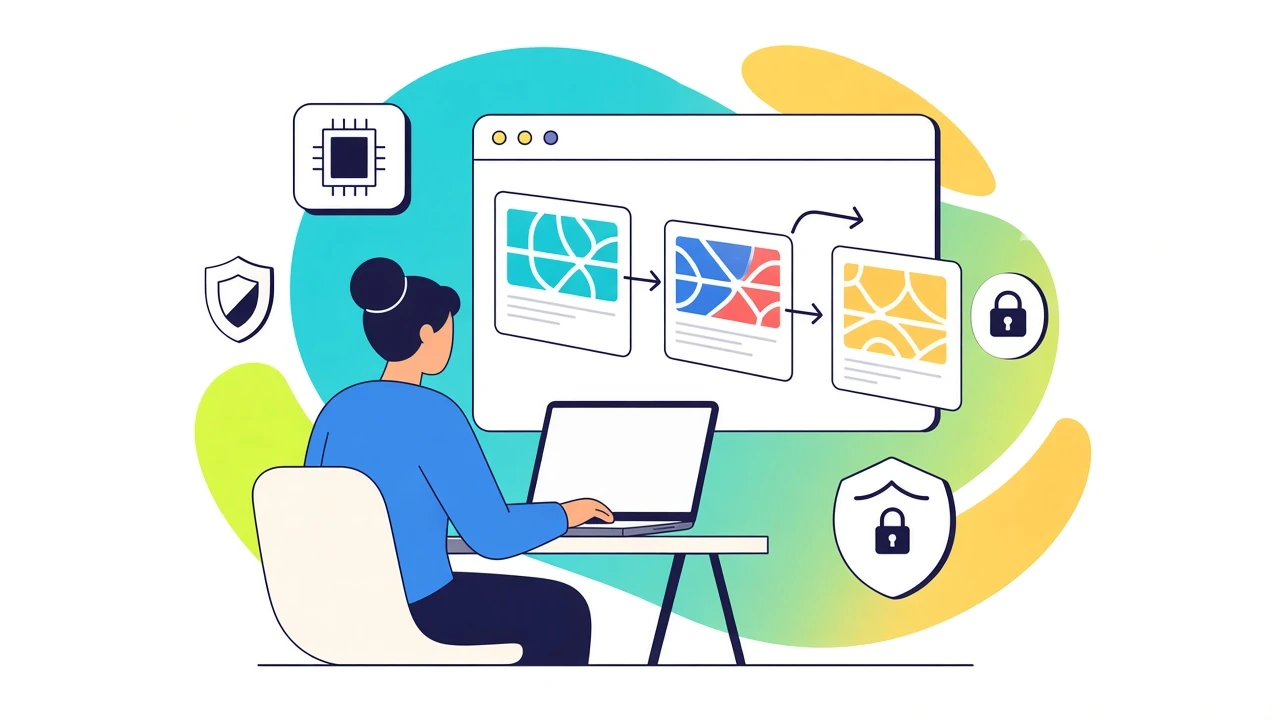
\includegraphics[width=\linewidth]{assets/solution.png}
  \caption*{\textbf{Réponse KORA.} Une couche locale traduit la surface
  accessible tout en isolant les valeurs sensibles.}
\end{minipage}
\end{figure}

KORA se place entre l’utilisateur et la représentation visuelle de la page.
Le service financier continue de calculer les frais, de gérer son formulaire
et de valider son parcours. L’extension ne remplace pas cette logique : elle
traduit uniquement les textes visibles qui passent ses contrôles.

\subsection{Cas d’usage principal}

\begin{enumerate}
  \item Amina ouvre l’interface Safinum en français ou en anglais.
  \item Elle ouvre la popup KORA et choisit \textbf{Fulfulde}.
  \item Le tableau de bord devient compréhensible en \code{fub}; le solde et
        le numéro de compte restent strictement identiques.
  \item Elle choisit une opération et saisit un montant. KORA traduit les
        libellés, mais le site conserve la valeur et calcule les frais.
  \item Elle saisit le nom, le téléphone, le motif et une note. Ces valeurs
        utilisateur ne sont pas traduites.
  \item Elle vérifie le récapitulatif, confirme et retrouve les mêmes valeurs
        sur le reçu puis sur le tableau de bord.
  \item Un message ou un écran ajouté après chargement repasse
        automatiquement dans le même pipeline de traduction.
\end{enumerate}

\begin{keybox}[Promesse utilisateur]
\textbf{Comprendre} l’action dans sa langue; \textbf{vérifier} les valeurs
canoniques sans altération; \textbf{confirmer} seulement lorsque le sens est
couvert. KORA privilégie la sûreté d’une interface partiellement traduite à la
fluidité trompeuse d’une interface entièrement générée.
\end{keybox}

\subsection{Interface et réversibilité}

\begin{figure}[H]
\centering
\begin{minipage}[c]{0.40\linewidth}
  \centering
  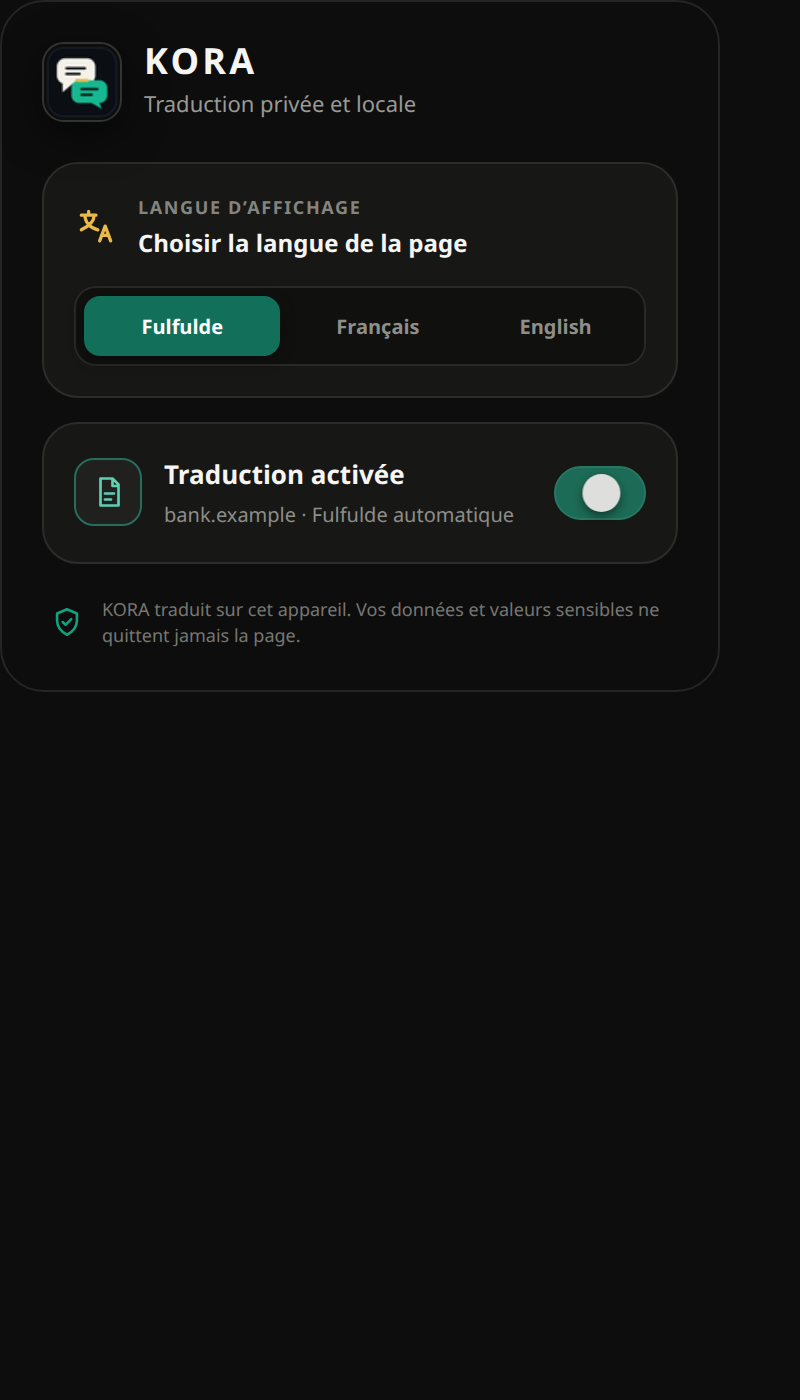
\includegraphics[width=0.72\linewidth]{assets/kora-popup.png}
\end{minipage}
\hfill
\begin{minipage}[c]{0.56\linewidth}
  \textbf{La popup pilote, elle ne traduit pas.}
  \begin{itemize}
    \item \textbf{Fulfulde} active la détection FR/EN et la sortie
          \code{fub}.
    \item \textbf{Français} ou \textbf{English} restaure d’abord les nœuds
          d’origine, puis déclenche le sélecteur natif du site lorsqu’il
          existe.
    \item L’interrupteur suspend ou reprend la traduction sans recharger le
          contenu.
    \item Après une action, la popup se ferme et rend le focus à la page;
          \code{Ctrl+A}, la tabulation et les raccourcis restent natifs.
  \end{itemize}
  \small
  KORA ne fabrique pas une traduction FR$\leftrightarrow$EN : ce changement
  dépend du contrôle linguistique du site. Son propre contrat est
  FR/EN$\rightarrow$\code{fub}.
\end{minipage}
\caption{Popup sombre KORA et comportement des trois choix de langue.}
\end{figure}

\subsection{Parcours financier démontré}

\begin{tikzpicture}[
  node distance=5mm and 4mm,
  journey/.style={draw=Line,fill=Paper,rounded corners=2mm,minimum height=18mm,
    text width=27mm,align=center,font=\small},
  num/.style={circle,fill=Teal,text=white,font=\bfseries,inner sep=2.2pt},
  arrow/.style={-{Latex[length=2.2mm]},thick,color=TealDark}
]
\node[journey] (s1) {\tikz\node[num]{1};\\[1mm]\textbf{Solde}\\compte et historique};
\node[journey,right=of s1] (s2) {\tikz\node[num]{2};\\[1mm]\textbf{Frais}\\type et montant};
\node[journey,right=of s2] (s3) {\tikz\node[num]{3};\\[1mm]\textbf{Bénéficiaire}\\données saisies};
\node[journey,right=of s3] (s4) {\tikz\node[num]{4};\\[1mm]\textbf{Récapitulatif}\\valeurs à vérifier};
\node[journey,right=of s4] (s5) {\tikz\node[num]{5};\\[1mm]\textbf{Confirmation}\\reçu et retour};
\draw[arrow] (s1) -- (s2);
\draw[arrow] (s2) -- (s3);
\draw[arrow] (s3) -- (s4);
\draw[arrow] (s4) -- (s5);
\end{tikzpicture}

Les erreurs \code{AMOUNT\_001}, \code{AMOUNT\_002},
\code{BENEFICIARY\_001}, \code{SECURITY\_001},
\code{SECURITY\_002}, \code{NETWORK\_001} et
\code{CONFIRM\_001} font partie de la matrice de contrôle. Les codes restent
intacts; leurs titres et explications visibles peuvent être traduits.

\subsection{Périmètre observable}

\begin{tabularx}{\linewidth}{@{}Y Y@{}}
\toprule
\textbf{Pris en charge} & \textbf{Hors exposition du navigateur}\\
\midrule
Nœuds texte; boutons; liens; labels; options visibles; \code{placeholder};
\code{aria-label}; \code{title}; contenu ajouté ou remplacé; Shadow DOM
ouvert; iframes autorisées. &
Texte incorporé à une image; pixels d’un \code{canvas}; Shadow DOM fermé;
pages \code{chrome://}; Chrome Web Store; iframe interdite par le navigateur.\\
\bottomrule
\end{tabularx}

Cette frontière est technique et vérifiable : une extension ne peut pas
traduire un texte que Chrome ne lui expose pas sans OCR, contournement ou
permission supplémentaire.

\section{Architecture et fonctionnement interne}

\subsection{Vue d’ensemble}

KORA suit une architecture locale à responsabilités séparées. La popup porte
l’intention de l’utilisateur; le content script observe la page; le moteur
décide si un segment peut être traduit; les modèles linguistiques classent
uniquement des formulations déjà autorisées. Le site cible demeure maître de
ses données et de sa logique métier.

\begin{figure}[H]
\centering
\resizebox{\linewidth}{!}{%
\begin{tikzpicture}[
  box/.style={draw=Line,fill=white,rounded corners=2mm,minimum height=12mm,
    minimum width=29mm,align=center,font=\small},
  core/.style={box,draw=Teal,fill=Mint},
  ext/.style={box,draw=InkSoft,fill=Paper},
  data/.style={draw=Gold,fill=Warm,rounded corners=2mm,minimum height=10mm,
    minimum width=28mm,align=center,font=\small},
  arrow/.style={-{Latex[length=2mm]},thick,color=TealDark},
  bi/.style={{Latex[length=2mm]}-{Latex[length=2mm]},thick,color=TealDark}
]
\node[ext] (user) {Utilisateur};
\node[core,right=13mm of user] (popup) {Popup\\activation · langue};
\node[data,below=7mm of popup] (storage) {Stockage local\\préférences seules};
\node[core,right=13mm of popup] (content) {Content script\\DOM · mutations};
\node[core,right=13mm of content] (engine) {Moteur\\sens · intégrité};
\node[data,above right=6mm and 10mm of engine] (mem) {Mémoires et\\gabarits FR/EN};
\node[data,right=10mm of engine] (spell) {Correcteur\\orthographique};
\node[data,below right=6mm and 10mm of engine] (model) {Modèles \code{fub}\\neuronal + n-gramme};
\node[ext,below=20mm of content] (page) {Page financière existante\\texte visible · formulaire · application};

\draw[bi] (user) -- (popup);
\draw[bi] (popup) -- node[above,font=\scriptsize]{messages Chrome} (content);
\draw[bi] (popup) -- (storage);
\draw[bi] (content) -- (storage);
\draw[bi] (content) -- node[above,font=\scriptsize]{segments} (engine);
\draw[bi] (content) -- node[left,font=\scriptsize]{lecture / rendu} (page);
\draw[bi] (engine) -- (mem);
\draw[bi] (engine) -- (spell);
\draw[bi] (engine) -- (model);
\end{tikzpicture}}
\caption{Architecture d’exécution : toutes les ressources linguistiques sont
embarquées dans l’extension.}
\end{figure}

\begin{evidencebox}[Absence de dépendance serveur]
Le bundle n’utilise aucune API de traduction, aucun proxy et aucun code
distant. La connexion Internet sert uniquement à charger le site financier
visité. Déconnecter le réseau après chargement ne change pas le pipeline KORA.
\end{evidencebox}

\subsection{Rôle précis de chaque composant}

\begin{longtable}{@{}|L{43mm}|L{58mm}|L{55mm}|@{}}
\hline
\textbf{Composant} & \textbf{Responsabilité} & \textbf{Contrat de sûreté}\\
\hline
\endfirsthead
\hline
\textbf{Composant} & \textbf{Responsabilité} & \textbf{Contrat de sûreté}\\
\hline
\endhead
\code{manifest.json} &
Déclare MV3, popup, icônes, content script et permissions. &
Pas de permission réseau ni de code distant.\\
\hline
\code{src/popup.*} &
Choix Fulfulde/Français/English, activation et état. &
Ne reçoit pas le contenu de page; rend le focus après action.\\
\hline
\code{src/content.js} &
Parcourt le DOM, collecte les valeurs, applique les sorties, restaure les
originaux et observe les mutations. &
Ne remplace pas les éléments interactifs; ne modifie aucune propriété de
formulaire.\\
\hline
\code{src/engine.js} &
Détection de source, cascade de traduction, couverture sémantique et contrôle
d’intégrité. &
Retourne l’original si le sens ou les valeurs échouent.\\
\hline
\code{src/spelling.js} &
Rapproche une entrée fautive d’une clé FR/EN connue avec distance
Damerau--Levenshtein bornée. &
Accepte seulement un meilleur sens unique; exclut nombres et codes.\\
\hline
\code{src/translations.js} &
Mémoire du parcours Safinum relue. &
Prioritaire sur les candidats terminologiques.\\
\hline
\texttt{src/general-\allowbreak translations.js} &
Libellés web et financiers généraux. &
Activé selon la langue et le contexte détectés.\\
\hline
\texttt{src/corpus-\allowbreak translations.js} &
Index FR/EN généré depuis 504 concepts. &
Conserve le statut de provenance et les codes protégés.\\
\hline
\code{src/language-model.js} &
Prédiction, score de fluidité et classement hybrides. &
Ne peut pas autoriser seul une traduction.\\
\hline
\texttt{src/neural-\allowbreak language-model.js} &
Inférence JavaScript des poids int8. &
Pas de bibliothèque d’inférence ni de chargement réseau.\\
\hline
\code{chrome.storage.local} &
Mémorise activation et langue choisie. &
Aucun texte de page, montant, nom ou historique.\\
\hline
\end{longtable}

\subsection{Séquence d’une activation}

\begin{figure}[H]
\centering
\begin{tikzpicture}[
  actor/.style={draw=Teal,fill=Mint,rounded corners=1.5mm,
    text width=22mm,minimum height=10mm,align=center,font=\small\bfseries},
  msg/.style={-{Latex[length=2mm]},line width=0.7pt,color=TealDark},
  life/.style={dashed,color=Line,thick}
]
\node[actor] (u) {Utilisateur};
\node[actor,right=11mm of u] (p) {Popup};
\node[actor,right=11mm of p] (c) {Content script};
\node[actor,right=11mm of c] (e) {Moteur};
\node[actor,right=11mm of e] (d) {Site};
\foreach \n in {u,p,c,e,d}
  \draw[life] (\n.south) -- ++(0,-78mm);
\draw[msg] ($(u.south)+(0,-8mm)$) -- node[above,font=\scriptsize]{choisit Fulfulde} ($(p.south)+(0,-8mm)$);
\draw[msg] ($(p.south)+(0,-18mm)$) -- node[above,font=\scriptsize]{active KORA} ($(c.south)+(0,-18mm)$);
\draw[msg] ($(c.south)+(0,-28mm)$) -- node[above,font=\scriptsize]{lit DOM et valeurs} ($(d.south)+(0,-28mm)$);
\draw[msg] ($(c.south)+(0,-38mm)$) -- node[above,font=\scriptsize]{segment protégé} ($(e.south)+(0,-38mm)$);
\draw[msg] ($(e.south)+(0,-48mm)$) -- node[above,font=\scriptsize]{sens et intégrité} ($(c.south)+(0,-48mm)$);
\draw[msg] ($(c.south)+(0,-58mm)$) -- node[above,font=\scriptsize]{texte visible traduit} ($(d.south)+(0,-58mm)$);
\draw[msg] ($(d.south)+(0,-68mm)$) -- node[above,font=\scriptsize]{nouveau contenu} ($(c.south)+(0,-68mm)$);
\end{tikzpicture}
\caption{La popup transmet le choix de langue; le content script lit et rend
le texte; le moteur contrôle le sens et l’intégrité sans modifier la logique du site.}
\end{figure}

\subsection{Pipeline de traduction contrôlée}

\begin{figure}[H]
\centering
\resizebox{0.97\linewidth}{!}{%
\begin{tikzpicture}[
  node distance=5mm and 7mm,
  action/.style={draw=Line,fill=Paper,rounded corners=1.5mm,
    text width=28mm,minimum height=11mm,align=center,font=\small},
  decision/.style={diamond,draw=Teal,fill=Mint,aspect=2.3,
    text width=25mm,align=center,font=\small,inner sep=1.5pt},
  safe/.style={action,draw=Teal,fill=Mint},
  stop/.style={action,draw=Gold,fill=Warm},
  arrow/.style={-{Latex[length=2mm]},thick,color=TealDark}
]
\node[action] (source) {Segment FR ou EN};
\node[decision,right=of source] (protected) {Valeur ou code protégé ?};
\node[action,right=of protected] (mask) {Masquer montants, dates, comptes et références};
\node[decision,right=of mask] (known) {Mémoire, faute unique, gabarit ou glossaire ?};
\node[safe,above right=8mm and 9mm of known] (candidate) {Candidat \code{fub} dont le sens est couvert};
\node[stop,below right=8mm and 9mm of known] (original) {Conserver l’original};
\node[decision,right=10mm of candidate] (coverage) {Couverture suffisante ?};
\node[action,right=of coverage] (rank) {Classement de fluidité};
\node[action,right=of rank] (restore) {Restaurer les valeurs};
\node[decision,right=of restore] (integrity) {Occurrences identiques ?};
\node[safe,right=of integrity] (render) {Rendre le texte};

\draw[arrow] (source) -- (protected);
\draw[arrow] (protected) -- node[above,font=\scriptsize]{non} (mask);
\draw[arrow] (protected) |- node[pos=.25,left,font=\scriptsize]{oui} (original);
\draw[arrow] (mask) -- (known);
\draw[arrow] (known) -- node[above left,font=\scriptsize]{oui} (candidate);
\draw[arrow] (known) -- node[below left,font=\scriptsize]{non} (original);
\draw[arrow] (candidate) -- (coverage);
\draw[arrow] (coverage) -- node[above,font=\scriptsize]{oui} (rank);
\draw[arrow] (coverage) |- node[pos=.25,right,font=\scriptsize]{non} (original);
\draw[arrow] (rank) -- (restore);
\draw[arrow] (restore) -- (integrity);
\draw[arrow] (integrity) -- node[above,font=\scriptsize]{oui} (render);
\draw[arrow] (integrity) |- node[pos=.25,right,font=\scriptsize]{non} (original);
\end{tikzpicture}}
\caption{La fluidité intervient après la détermination du sens et avant le
dernier contrôle d’intégrité.}
\end{figure}

Ordre de décision : mémoire Safinum exacte; mémoire web/finance générale;
terminologie contrôlée; correction orthographique non ambiguë; gabarit typé;
phrasebook par correspondance longue; abstention. Pour un message financier
critique, la couverture requise est de 100\,\%; elle est de 80\,\% pour un
segment non critique, sous réserve du verrou d’intégrité.

\subsection{Contenu dynamique}

\begin{figure}[H]
\centering
\resizebox{\linewidth}{!}{%
\begin{tikzpicture}[
  node distance=4.5mm,
  flow/.style={draw=Line,fill=Paper,rounded corners=1.5mm,
    minimum height=10mm,text width=29mm,align=center,font=\small},
  arrow/.style={-{Latex[length=2mm]},thick,color=TealDark}
]
\node[flow] (mut) {Mutation DOM ou événement utilisateur};
\node[flow,right=of mut] (deb) {Regroupement court des changements};
\node[flow,right=of deb] (disc) {Découverte du document et des racines ouvertes};
\node[flow,right=of disc] (class) {Classement : source ou valeur protégée};
\node[flow,right=of class] (trans) {Même pipeline de traduction};
\node[flow,right=of trans] (apply) {Mise à jour idempotente du texte};
\draw[arrow] (mut)--(deb);
\draw[arrow] (deb)--(disc);
\draw[arrow] (disc)--(class);
\draw[arrow] (class)--(trans);
\draw[arrow] (trans)--(apply);
\end{tikzpicture}}
\caption{Traitement des contenus ajoutés après le chargement de la page.}
\end{figure}

Le content script combine \code{MutationObserver}, les événements
\code{click}/\code{change}/\code{input} et un rescan de sûreté toutes les
500\,ms lorsque l’onglet est visible. Il prend en charge les écrans montés par
framework, les frais recalculés, les erreurs, les attributs et les options,
sans remplacer le composant d’origine.

\subsection{Construction et artefacts}

\begin{figure}[H]
\centering
\resizebox{\linewidth}{!}{%
\begin{tikzpicture}[
  node distance=5mm and 7mm,
  b/.style={draw=Line,fill=Paper,rounded corners=1.5mm,
    minimum height=10mm,text width=27mm,align=center,font=\small},
  artifact/.style={b,draw=Teal,fill=Mint},
  arrow/.style={-{Latex[length=2mm]},thick,color=TealDark}
]
\node[b] (src) {Sources JS, données et manifest};
\node[b,right=of src] (term) {Compilation terminologique};
\node[b,right=of term] (bundle) {Bundle esbuild + ressources};
\node[artifact,right=of bundle] (unpacked) {\code{kora-unpacked/}};
\node[artifact,above right=5mm and 7mm of unpacked] (zip) {{\ttfamily\scriptsize kora-\\extension.zip}};
\node[artifact,below right=5mm and 7mm of unpacked] (json) {Modèle JSON exportable};
\draw[arrow] (src)--(term);
\draw[arrow] (term)--(bundle);
\draw[arrow] (bundle)--(unpacked);
\draw[arrow] (unpacked)--(zip);
\draw[arrow] (bundle)|-(json);
\end{tikzpicture}}
\caption{Chaîne de build : le packaging échoue si l’archive dépasse 10 Mio.}
\end{figure}

Le ZIP final ne contient ni corpus brut, ni PyTorch, ni Puppeteer, ni clé
secrète. Il contient le manifest, la popup, les icônes et les bundles où sont
déjà intégrés moteur, mémoires et poids KORA.

\section{Sécurité, intégrité et accessibilité}

\subsection{Modèle de menace}

Le risque principal n’est pas l’interception d’une requête de traduction :
KORA n’en émet aucune. Le risque est une modification silencieuse du sens ou
d’une valeur canonique pendant le rendu. La conception traite donc la
traduction comme une transformation non fiable qui doit prouver qu’elle a
conservé les données.

\begin{tabularx}{\linewidth}{@{}|L{40mm}|Y|Y|@{}}
\hline
\textbf{Risque} & \textbf{Impact possible} & \textbf{Mesure KORA}\\
\hline
Montant ou devise altéré &
Décision financière erronée &
Masquage, restauration exacte, comptage des occurrences, rejet.\\
\hline
Bénéficiaire traduit &
Confusion sur le destinataire &
Noms et valeurs saisies ajoutés au jeu protégé en mémoire d’onglet.\\
\hline
Action inversée &
Confirmer au lieu d’annuler, créditer au lieu de débiter &
Actions critiques en mémoire exacte; négation inconnue = abstention.\\
\hline
Alerte affaiblie &
Utilisateur insuffisamment averti &
Messages complets, seuil de couverture critique à 100\,\%.\\
\hline
Fuite de contenu &
Exposition de données personnelles &
Pas de transport réseau, télémétrie ou stockage persistant de page.\\
\hline
Régression d’interface &
Clavier ou formulaire inutilisable &
Modification des nœuds textuels, pas des composants ou de leur ordre.\\
\hline
\end{tabularx}

\subsection{Invariant d’intégrité}

Soit \(P(s)\) le multiensemble des valeurs protégées extraites d’un segment
source \(s\), et \(t\) une traduction candidate. KORA accepte \(t\) seulement
si :

\[
  \forall v \in P(s),\quad
  \operatorname{occ}(v,s)=\operatorname{occ}(v,t)
  \quad\text{et}\quad
  \operatorname{bytes}(v_s)=\operatorname{bytes}(v_t).
\]

En pratique, les valeurs sont remplacées temporairement par des jetons
internes, par exemple \code{<<KORA\_0>>}, puis remises caractère pour caractère.
Le contrôle final protège aussi les répétitions : une valeur ne doit ni
disparaître, ni être dupliquée.

\begin{keybox}[Exemple de transformation sûre]
\textbf{Source :} Votre transfert de \texttt{25 000 FCFA} est en attente.\\
\textbf{Interne :} Votre transfert de \texttt{<<KORA\_0>>} est en attente.\\
\textbf{Candidat :} Transfeer maa \texttt{<<KORA\_0>>} ɗon e fadde.\\
\textbf{Rendu :} Transfeer maa \texttt{25 000 FCFA} ɗon e fadde.
\end{keybox}

\subsection{Données protégées}

\begin{multicols}{2}
\begin{itemize}
  \item montants, signes et séparateurs;
  \item monnaies et pourcentages;
  \item comptes et numéros de téléphone;
  \item références et codes d’erreur;
  \item dates, heures, URL et courriels;
  \item noms complets et valeurs utilisateur.
\end{itemize}

\columnbreak
\begin{itemize}
  \item \code{input.value} et \code{textarea.value};
  \item \code{select.value} et valeur technique d’une option;
  \item \code{checked}, \code{selected}, \code{name}, \code{id};
  \item \code{type}, \code{min}, \code{step};
  \item contenu \code{contenteditable};
  \item identifiants opaques comme \code{DSAFDF}.
\end{itemize}
\end{multicols}

Dans un \code{select}, seul le libellé visible d’une option peut changer.
Sa valeur technique reste intacte. Le texte saisi
\texttt{Payment for services} reste lui aussi intact, même si le label du
champ est traduit.

\subsection{Cycle de vie des données}

\begin{figure}[H]
\centering
\begin{tikzpicture}[
  node distance=6mm and 12mm,
  b/.style={draw=Line,fill=Paper,rounded corners=1.5mm,
    text width=31mm,minimum height=11mm,align=center,font=\small},
  ok/.style={b,draw=Teal,fill=Mint},
  no/.style={b,draw=Gold,fill=Warm},
  arrow/.style={-{Latex[length=2mm]},thick,color=TealDark}
]
\node[b] (read) {Lecture temporaire du segment visible};
\node[b,right=of read] (protect) {Extraction des valeurs et masquage};
\node[b,right=of protect] (translate) {Traitement local en mémoire};
\node[ok,right=of translate] (render) {Rendu du texte ou original};
\node[no,below=9mm of protect] (store) {Jamais écrit dans le stockage};
\node[no,below=9mm of translate] (network) {Jamais envoyé sur le réseau};
\draw[arrow] (read)--(protect);
\draw[arrow] (protect)--(translate);
\draw[arrow] (translate)--(render);
\draw[-{Latex[length=2mm]},thick,color=Risk] (protect)--(store);
\draw[-{Latex[length=2mm]},thick,color=Risk] (translate)--(network);
\end{tikzpicture}
\caption{Le contenu financier reste dans la mémoire volatile de l’onglet.}
\end{figure}

\code{chrome.storage.local} conserve uniquement la préférence d’activation et
la langue d’affichage. Le jeu de valeurs utilisateur, utilisé pour reconnaître
le même nom ou la même note au récapitulatif, existe uniquement en mémoire du
content script et disparaît avec l’onglet.

\subsection{Permissions et indépendance}

\begin{lstlisting}[language={},caption={Permissions déclarées dans manifest.json}]
"permissions": ["storage", "activeTab", "scripting"]
\end{lstlisting}

\begin{itemize}
  \item \code{storage} conserve les préférences non sensibles.
  \item \code{activeTab} relie la popup à l’onglet explicitement utilisé.
  \item \code{scripting} charge le moteur local si l’onglet ne possède pas
        encore le protocole courant.
\end{itemize}

Le content script est déclaré pour les pages ordinaires HTTP, HTTPS et fichiers
locaux. Cette portée démontre l’indépendance par rapport à Safinum, mais KORA
ne contourne ni politique de contenu, ni iframe interdite, ni page interne
Chrome.

\subsection{Accessibilité et expérience utilisateur}

\begin{tabularx}{\linewidth}{@{}|L{43mm}|Y|@{}}
\hline
\textbf{Principe} & \textbf{Application}\\
\hline
Navigation clavier &
Aucun gestionnaire global ne bloque \code{Ctrl+A}; tabulation et commandes du
site sont conservées.\\
\hline
Focus &
La popup possède des styles de focus visibles et se ferme après action pour
rendre le focus à la page.\\
\hline
Sémantique &
Les éléments ne sont ni clonés ni remplacés; rôles, labels et ordre DOM
restent ceux du site.\\
\hline
Lecteurs d’écran &
\code{aria-label}, \code{title} et \code{placeholder} peuvent être traduits;
les sorties portent \code{lang="fub"}.\\
\hline
Lisibilité &
Popup sombre, contrastes élevés, contrôles dimensionnés et états explicites.\\
\hline
Réversibilité &
Chaque nœud conserve sa forme source; l’utilisateur peut restaurer la page
instantanément.\\
\hline
\end{tabularx}

\subsection{Cadre de démonstration}

Toutes les opérations sont simulées. Les comptes, noms, numéros, montants et
références du parcours servent uniquement à vérifier l’intégrité; KORA ne
déclenche aucun transfert et ne doit recevoir aucune donnée bancaire réelle.
La démonstration respecte la page fournie : elle charge l’extension comme une
extension utilisateur, sans modifier le code source ni contourner les étapes.

\begin{warningbox}[Limite réglementaire]
KORA est un prototype d’accessibilité, pas un dispositif bancaire certifié,
un outil d’autorisation de transaction ou un conseil financier. Un déploiement
réel exigerait une revue de sécurité indépendante, une double validation
linguistique, des essais utilisateurs et la gouvernance versionnée du
glossaire.
\end{warningbox}

\section{Langue, corpus et modèles embarqués}

\subsection{Variété cible et méthode linguistique}

KORA cible le \textbf{fulfulde de l’Adamaoua}, code ISO 639-3
\code{fub}, en écriture latine. Les caractères \texttt{ɓ}, \texttt{ɗ},
\texttt{ƴ}, \texttt{ŋ} et \texttt{ɲ} sont conservés en UTF-8. Les corpus
étiquetés \code{ff}, \code{fuv}, \code{fuf} ou \code{ffm} ne sont pas
silencieusement assimilés à cette variété camerounaise.

\begin{figure}[H]
\centering
\begin{minipage}[c]{0.47\linewidth}
  
\includegraphics[width=\linewidth]{assets/validation.png}
\end{minipage}
\hfill
\begin{minipage}[c]{0.49\linewidth}
  \textbf{Processus appliqué à une entrée critique}
  \begin{enumerate}
    \item identifier le concept financier en FR et EN;
    \item rechercher une forme camerounaise \code{fub};
    \item recouper l’orthographe et le contexte;
    \item distinguer attestation, emprunt et composition;
    \item vérifier que FR et EN donnent la même sortie;
    \item tester les valeurs, négations et actions;
    \item enregistrer source, statut et décision.
  \end{enumerate}
\end{minipage}
\caption{Validation humaine, traçabilité et contrôles automatisés sont
complémentaires.}
\end{figure}

\textbf{\LinguisticValidator} assure la responsabilité de la validation
linguistique du projet. Les formulations historiques relues sont distinguées
des propositions compositionnelles encore à valider. Cette séparation évite
de présenter une génération de corpus comme une norme linguistique.

\subsection{Sources et propriété intellectuelle}

\begin{longtable}{@{}L{43mm}L{29mm}L{43mm}L{37mm}@{}}
\toprule
\textbf{Ressource} & \textbf{Licence} & \textbf{Usage KORA} &
\textbf{Redistribution}\\
\midrule
\endfirsthead
\toprule
\textbf{Ressource} & \textbf{Licence} & \textbf{Usage KORA} &
\textbf{Redistribution}\\
\midrule
\endhead
Common Voice 27 \code{fub} &
CC0 &
1\,067 phrases pour orthographe et modèle de fluidité &
Pas de corpus brut dans l’extension.\\
Tourneux \& Konaï, vocabulaire mobile &
CC BY 4.0 &
Terminologie camerounaise des communications et transferts &
Attribution conservée.\\
Ressources SIL \code{fub} &
Conditions propres &
Consultation et contrôle, sans extraction automatisée &
Non redistribuées.\\
Deux inventaires financiers fournis &
Licence non déclarée &
Inventaire de concepts et définitions françaises &
Fichiers conservés dans le dépôt; pas présentés comme corpus parallèle.\\
PanLex \code{fub} &
Ambiguïté de licence / restriction non commerciale &
Évalué, non intégré &
Non redistribué.\\
Google Translate vers \code{ff} &
Service externe de comparaison &
Cinq réponses publiques comparées; aucune importation automatique &
Résultats archivés séparément.\\
Code KORA &
MIT &
Extension, moteur, modèles et tests &
Distribué sous MIT.\\
\bottomrule
\end{longtable}

\subsection{Inventaires financiers et statuts}

Les deux volumes fournis totalisent 2\,859 lignes et 512 libellés, ramenés à
504 concepts après déduplication de huit chevauchements. Ils décrivent les
concepts en français, mais ne constituent pas une vérité parallèle
FR/EN$\rightarrow$\code{fub}. La matrice synthétique finale du volume 2 est
exclue : elle contient notamment des associations contradictoires entre
réussites et causes d’échec.

\begin{tabularx}{\linewidth}{@{}L{47mm}C{22mm}Y@{}}
\toprule
\textbf{Statut} & \textbf{Nombre} & \textbf{Interprétation}\\
\midrule
\code{reviewed-existing} & 20 &
Formulation déjà présente dans la mémoire KORA relue.\\
\code{compositional-candidate} & 340 &
Composition transparente mais encore à confirmer par revue native.\\
\code{local-loan-candidate} & 31 &
Emprunt technique cohérent avec l’usage local, à confirmer.\\
\code{preserved-code} & 113 &
Code ou identifiant qui reste strictement identique.\\
\midrule
\textbf{Total} & \textbf{504} & 391 clés françaises et 390 clés anglaises.\\
\bottomrule
\end{tabularx}

Les candidats élargissent la reconnaissance de l’interface et alimentent le
modèle à poids réduit, mais leur statut demeure visible. Ils ne remplacent pas
une attestation indépendante.

\subsection{Corrections morphologiques intégrées}

La revue du 14 novembre 2026 a corrigé des faux-sens et harmonisé les noms
d’action. Les concepts emploient préférentiellement la forme nominale
\texttt{-ugol}; une commande peut garder la forme verbale Adamawa en
\texttt{-ugo}.

\begin{tabularx}{\linewidth}{@{}L{38mm}L{49mm}Y@{}}
\toprule
\textbf{Concept} & \textbf{Forme retenue} & \textbf{Décision}\\
\midrule
Compte bloqué & \texttt{Konte uddaaɗo} &
Participe passé adjectival, pas verbe conjugué.\\
Date de valeur & \texttt{Ñalngu kiisaangu} &
Écarte le faux-sens «\,ancien/usé\,».\\
Découvert autorisé & \texttt{Kaalisi ɓeydaaɗi yamiraaɗi} &
Accord avec la classe de \texttt{kaalisi}.\\
Paiement récurrent & \texttt{Yoɓugol lortotoongol} &
Écarte le sens «\,défaire/résilier\,».\\
Paiement sans contact & \texttt{Yoɓugol tawa meemaaka} &
Voyelle longue de \texttt{meemugo}.\\
Remboursement de prêt & \texttt{Yoɓugol nyamaande} &
Sens dette/prêt explicite.\\
Remboursement marchand & \texttt{Ruttinangol kaalisi} &
Restitution d’argent distincte du prêt.\\
Rétrofacturation & \texttt{Ruttinangol kaalisi yoɓaaɗi} &
Nom d’action et objet financier explicites.\\
\bottomrule
\end{tabularx}

\subsection{Pourquoi plusieurs couches plutôt qu’un traducteur génératif}

Deux modèles téléchargeables ont été évalués sur cinq actions critiques :
Flagship \code{francais-fufulde} et DS4H \code{linguo\_mt\_en\_fub}. Les
sorties observées comportaient répétitions, omissions ou contresens; leurs
empreintes dépassaient aussi la limite de 10 Mio. NLLB-200 et M2M-100 sont
beaucoup plus volumineux et ne ciblent pas précisément \code{fub}.

KORA sépare donc le \textbf{sens} de la \textbf{fluidité}. Le moteur
déterministe choisit un concept et protège ses valeurs. Les modèles
linguistiques embarqués ne voient ensuite que des formulations \code{fub}
déjà sûres, qu’ils peuvent classer mais jamais autoriser seuls.

\subsection{Architecture du modèle neuronal}

\begin{figure}[H]
\centering
\resizebox{\linewidth}{!}{%
\begin{tikzpicture}[
  node distance=6mm,
  b/.style={draw=Line,fill=Paper,rounded corners=1.5mm,text width=30mm,
    minimum height=12mm,align=center,font=\small},
  m/.style={b,draw=Teal,fill=Mint},
  arrow/.style={-{Latex[length=2mm]},thick,color=TealDark}
]
\node[b] (ctx) {Trois mots précédents};
\node[m,right=of ctx] (emb) {Embeddings\\24 dimensions};
\node[m,right=of emb] (hid) {Couche tanh\\96 neurones};
\node[m,right=of hid] (out) {Distribution du mot suivant\\vocabulaire 1\,472};
\node[b,below=9mm of hid] (ng) {Trigrammes, bigrammes et unigrammes};
\node[m,right=of out] (rank) {Prédiction et score de fluidité};
\draw[arrow] (ctx)--(emb);
\draw[arrow] (emb)--(hid);
\draw[arrow] (hid)--(out);
\draw[arrow] (out)--(rank);
\draw[arrow] (ng)-|(rank);
\end{tikzpicture}}
\caption{Réseau KORA quantifié et repli n-gramme déterministe.}
\end{figure}

\begin{tabularx}{\linewidth}{@{}L{50mm}Y@{}}
\toprule
\textbf{Caractéristique} & \textbf{Valeur reproductible}\\
\midrule
Architecture & Contexte 3, embedding 24, tanh 96\\
Paramètres & 185\,120\\
Quantification & Poids int8; biais float32\\
Vocabulaire neuronal & 1\,472 unités\\
Données d’entraînement &
1\,067 phrases Common Voice; 9\,368 tokens; 262 formulations KORA;
386 formulations terminologiques à poids réduit\\
Repli n-gramme & 1\,199 mots fréquents; 1\,561 contextes\\
Validation tenue à part & 107 phrases Common Voice\\
Résultat int8 & top-1 14,8\,\%; top-5 35,0\,\%\\
Entraînement & Graine 2026; meilleur état époque 2; arrêt après 8/40\\
Taille générée & Environ 262 Kio avec vocabulaire et métadonnées\\
\bottomrule
\end{tabularx}

La configuration retenue maximise la top-5 parmi les variantes évaluées,
métrique cohérente avec un rôle de classement de plusieurs candidats. Le
score du mot suivant fusionne 85\,\% de réseau et 15\,\% de n-gramme; le score
de phrase combine ensuite 80\,\% de score neuronal et 20\,\% de score
n-gramme. Un cache borné garde les 1\,000 derniers scores.

\begin{warningbox}[Ce que le modèle ne fait pas]
Le modèle de langue n’est pas un traducteur FR/EN autonome. Il ne connaît pas
les règles de conservation financière et ne doit pas être appelé seul pour
produire un message bancaire. La fonction \code{translateText} orchestre la
mémoire, le correcteur, les gabarits, le modèle et le verrou d’intégrité.
\end{warningbox}

\subsection{Preuve d’usage dans l’extension}

\begin{enumerate}
  \item \code{translateText} obtient un candidat dont le sens et les valeurs
        sont déjà contrôlés;
  \item \code{scoreFubFluency} appelle \code{scoreNeuralFub};
  \item l’inférence JavaScript décode les poids int8 et calcule les
        probabilités;
  \item le n-gramme complète les séquences peu vues;
  \item \code{rankFubCandidates} trie uniquement ces candidats sûrs;
  \item le contrôle d’intégrité peut encore rejeter le résultat.
\end{enumerate}

Le fichier \code{src/fub-neural-model.js} est regroupé dans
\code{content.js} au build. Il n’est ni téléchargé au premier démarrage, ni
simulé par une métadonnée. \code{npm run model:demo} et les tests unitaires
appellent les mêmes poids que le bundle Chrome.

\section{Validation, tests et preuves}

\subsection{Stratégie de preuve}

La validation suit le risque : les unités vérifient chaque invariant; les
tests de page reproduisent le DOM, les mutations et la popup; les tests live
chargent réellement l’extension dans Chrome et parcourent une interface
distante. Une vérification manuelle complète les aspects difficiles à
automatiser, notamment zoom, contraste et lecture d’écran.

\begin{figure}[H]
\centering
\begin{tikzpicture}[
  level/.style={trapezium,trapezium left angle=75,trapezium right angle=105,
    draw=Line,minimum height=11mm,align=center,font=\small},
]
\node[level,fill=Mint,minimum width=56mm] (l1) at (0,0)
  {\textbf{Tests live}\\Safinum + UBA dans Chrome};
\node[level,fill=Paper,minimum width=89mm] (l2) at (0,-12mm)
  {\textbf{Tests navigateur}\\popup · mutations · iframe · Shadow DOM};
\node[level,fill=Warm,minimum width=124mm] (l3) at (0,-24mm)
  {\textbf{Tests unitaires et corpus}\\moteur · intégrité · orthographe · modèles · export};
\end{tikzpicture}
\caption{Pyramide de test KORA : précision en bas, parcours réel en haut.}
\end{figure}

\subsection{Résultat automatisé de référence}

Le 14 novembre 2026, la suite cœur a reconstruit les index puis exécuté
27 tests :

\begin{keybox}[Résultat observé]
\texttt{tests 27 · pass 27 · fail 0 · skipped 0}\\
Durée du runner : environ 9,53 s; durée avec précompilation : 15,60 s.\\
Index généré : 504 entrées, 391 clés FR, 390 clés EN.
\end{keybox}

Cette suite couvre notamment les sept erreurs publiques, la parité FR/EN, les
valeurs canoniques, les phrases inédites compositionnelles, l’abstention, les
corrections morphologiques, l’export du modèle et une faute générée pour chaque
libellé éligible.

\subsection{Commandes reproductibles}

\begin{lstlisting}[language=bash]
npm install
npm test                 # moteur, corpus, modèles, export, orthographe
npm run test:spelling    # 1 252 libellés fautifs FR/EN
npm run test:popup       # protocole, thème, activation, restauration
npm run test:pages       # DOM dynamique, attributs, iframe, Shadow DOM
npm run test:live        # parcours Safinum réel dans Chrome
npm run test:uba         # page UBA réelle et Ctrl+A
npm run test:all         # chaîne complète
npm run package          # rebuild, modèle exporté, ZIP < 10 Mio
\end{lstlisting}

\subsection{Matrice des scénarios critiques}

\begin{longtable}{@{}L{43mm}L{55mm}L{57mm}@{}}
\toprule
\textbf{Scénario} & \textbf{Oracle} & \textbf{Couverture}\\
\midrule
\endfirsthead
\toprule
\textbf{Scénario} & \textbf{Oracle} & \textbf{Couverture}\\
\midrule
\endhead
Source française / anglaise &
Même intention source, même sortie \code{fub}. &
Tests moteur et bascule live.\\
Solde et historique &
Montants, signes, dates et devise identiques. &
Tests moteur + tableau de bord live.\\
Calcul des frais &
Montant, frais et total identiques avant/après traduction. &
Tests valeurs + étape frais live.\\
Données bénéficiaire &
Nom, téléphone, motif et note inchangés. &
Tests formulaire, récapitulatif et reçu.\\
Libellé d’un \code{select} &
Texte visible traduit; valeur technique inchangée. &
Test navigateur dédié.\\
Message ajouté après chargement &
Détecté par l’observateur et traité sans hook. &
Ajout, \code{innerHTML}, fragment, remplacement, attribut.\\
Fautes d’orthographe &
Même sortie uniquement si un meilleur sens est unique. &
1\,252 libellés : 628 FR et 624 EN.\\
Texte libre inconnu &
Source conservée; aucune phrase inventée. &
Test de faible confiance.\\
Négation financière inconnue &
Source conservée. &
\texttt{Le transfert n'a pas échoué.}\\
Code technique &
Code conservé; explication visible traduisible. &
HTTP, événements, API et erreurs Safinum.\\
Sélection clavier &
\code{Ctrl+A} sélectionne la page et un champ normalement. &
Tests popup, pages et UBA.\\
Restauration &
Tous les nœuds reviennent à leur texte original. &
Test protocole popup/content script.\\
\bottomrule
\end{longtable}

\subsection{Test live Safinum}

Le scénario automatisé ouvre Chrome avec \code{kora-unpacked}, puis :

\begin{enumerate}
  \item active KORA sur l’environnement Safinum;
  \item vérifie le tableau de bord et les valeurs canoniques;
  \item ajoute après chargement des messages connus, fautifs et variables;
  \item consulte les frais et choisit le type d’opération;
  \item saisit des données fictives de bénéficiaire;
  \item vérifie le récapitulatif et confirme;
  \item contrôle le reçu, la référence et le retour au tableau de bord;
  \item ouvre une seconde page, bascule Safinum en anglais et confirme la
        même sortie \code{fub}.
\end{enumerate}

Le résultat de référence documenté est :

\begin{lstlisting}[language={}]
LIVE PASS: French journey, dynamic content, form values and receipt integrity.
LIVE PASS: English source switched and translated to the same fub interface.
\end{lstlisting}

Le contrôle UBA est facultatif et dépend d’un site tiers. Une exécution
antérieure a vérifié la sélection de page et de champ; lors de la vérification
finale du 14 novembre, la navigation vers ce site a expiré après 90 secondes.
Ce résultat n’est donc pas présenté comme une réussite reconfirmée.

\subsection{Tests du correcteur orthographique}

Le correcteur normalise accents et ponctuation puis autorise de une à quatre
opérations selon la longueur : insertion, suppression, substitution ou
inversion adjacente. Les tests génèrent une variante fautive pour chaque clé
textuelle éligible et exigent exactement la traduction de la clé d’origine.

\begin{tabularx}{\linewidth}{@{}L{39mm}L{50mm}Y@{}}
\toprule
\textbf{Entrée} & \textbf{Sortie attendue} & \textbf{Règle}\\
\midrule
\texttt{sodle insufisant} &
\texttt{Kaalisi yonaa} &
Deux fautes, rapprochement unique.\\
\texttt{insuficient balnce} &
\texttt{Kaalisi yonaa} &
Source anglaise fautive, intention connue.\\
Deux clés également proches &
Texte source &
Ambiguïté = abstention.\\
\texttt{NETWORK\_001} &
\texttt{NETWORK\_001} &
Code protégé, jamais corrigé approximativement.\\
\bottomrule
\end{tabularx}

\subsection{Évaluation du modèle de langue}

La validation neuronale est séparée par phrase : 107 phrases Common Voice ne
participent pas à l’entraînement. Les 262 formulations KORA et 386 candidats
terminologiques enrichissent l’entraînement mais ne gonflent pas cette
métrique. \code{npm run model:demo} vérifie directement les poids livrés :

\begin{lstlisting}[language={}]
transfeer maa -> yettaama, neldaama
kaalisi       -> gondi, yonaa
Votre paiement de 25 000 FCFA a ete refuse.
-> Yobugol maa 25 000 FCFA salaama.
Le transfert n'a pas echoue.
-> original conserve
\end{lstlisting}

Les caractères ASCII de cet extrait simplifient l’affichage du terminal;
l’exécution réelle et les fichiers utilisent l’orthographe UTF-8 complète.

\subsection{Contrôles manuels avant remise}

\begin{itemize}
  \item types d’opération : compte Safinum, Mobile Money, autre banque;
  \item montants : zéro, 25\,000, supérieur au solde, seuils de frais;
  \item erreurs : montant, bénéficiaire, sécurité, réseau et confirmation;
  \item clavier seul, focus visible, zoom 200\,\%, contraste et lecteur d’écran;
  \item activation, suspension, restauration, rechargement et changement
        FR/EN;
  \item vérification visuelle du reçu puis retour au tableau de bord.
\end{itemize}

\begin{warningbox}[Interprétation des preuves]
Les tests établissent l’intégrité du logiciel sur les cas couverts. Ils ne
transforment pas automatiquement chaque proposition terminologique en forme
native validée. La preuve technique et la preuve linguistique restent
séparées et sont toutes deux nécessaires avant production.
\end{warningbox}

\section{Installation, intégration et reproduction}

\subsection{Installer le prototype livré}

Chrome ne charge pas directement une archive ZIP. La procédure reproductible
est :

\begin{enumerate}
  \item décompresser \code{release/kora-extension.zip}, ou utiliser directement
        \code{release/kora-unpacked};
  \item ouvrir \code{chrome://extensions};
  \item activer \textbf{Mode développeur};
  \item cliquer \textbf{Charger l’extension non empaquetée};
  \item sélectionner le dossier qui contient directement
        \code{manifest.json};
  \item ouvrir ou actualiser la page financière;
  \item épingler KORA, ouvrir sa popup et choisir \textbf{Fulfulde}.
\end{enumerate}

\begin{keybox}[Démonstration minimale en moins d’une minute]
Vérifier d’abord un montant et un compte sur la page source. Activer Fulfulde,
constater que les libellés changent mais que les valeurs restent identiques.
Changer d’étape, provoquer une erreur simulée, puis choisir Français ou
English pour restaurer la page.
\end{keybox}

\subsection{Construire depuis les sources}

\textbf{Prérequis :} Node.js 20 ou supérieur, npm, Python 3 et Google Chrome.
PyTorch et NumPy sont nécessaires uniquement pour réentraîner le réseau; les
poids versionnés suffisent pour construire et tester l’extension.

\begin{lstlisting}[language=bash]
git clone https://github.com/kaezerwatto/KORA.git
cd KORA
npm install
npm run build
npm test
npm run package
\end{lstlisting}

\code{npm run package} reconstruit la terminologie, regroupe le bundle,
exporte le modèle JSON, produit le dossier unpacked et crée le ZIP. Le script
interrompt la livraison au-delà de 10 Mio.

\subsection{Régénérer les ressources linguistiques}

\begin{lstlisting}[language=bash]
npm run build:corpora       # inventaire et empreintes des deux volumes
npm run build:terminology   # index FR/EN -> fub et codes proteges
npm run build:model         # modele n-gramme
npm run model:train         # reseau, early stopping, int8
npm run model:export        # JSON portable + empreinte SHA-256
npm run model:demo          # predictions et cas d'abstention
\end{lstlisting}

L’entraînement écrit \code{src/fub-neural-model.js}; le build l’embarque dans
\code{content.js}. L’export indépendant est
\code{release/kora-fub-neural-model.json}. Il contient architecture,
vocabulaire, tenseurs int8 encodés, échelles et empreinte de contrôle, mais
aucun contenu utilisateur.

\subsection{Utiliser le moteur complet séparément}

Dans un projet JavaScript ESM, importer \code{translateText}. Cette API porte
la protection des valeurs et convient à une traduction contrôlée :

\begin{lstlisting}[language={}]
import { translateText } from "./src/engine.js";

const result = translateText("sodle insufisant", {
  sourceHint: "fr",
  domainHint: "financial",
  protectedValues: []
});

console.log(result.text);    // Kaalisi yonaa
console.log(result.method);  // spelling-memory
\end{lstlisting}

\begin{tabularx}{\linewidth}{@{}L{38mm}Y@{}}
\toprule
\textbf{Option/résultat} & \textbf{Signification}\\
\midrule
\code{sourceHint} & \code{auto}, \code{fr} ou \code{en}.\\
\code{domainHint} & \code{general} ou \code{financial}.\\
\code{protectedValues} & Chaînes à conserver strictement.\\
\code{text} & Traduction acceptée ou texte original.\\
\code{changed} & Indique si le rendu a changé.\\
\code{method} &
\code{memory}, \code{spelling-memory}, \code{template},
\code{glossary}, \code{protected}, \code{integrity-fallback} ou
\code{original}.\\
\code{fluency} & Score du modèle lorsque pertinent.\\
\bottomrule
\end{tabularx}

\subsection{Utiliser uniquement les modèles de langue}

\begin{lstlisting}[language={}]
import {
  predictNextFub,
  rankFubCandidates,
  scoreFubFluency
} from "./src/language-model.js";

predictNextFub("transfeer maa", 5);
scoreFubFluency("Kaalisi yonaa");
rankFubCandidates([
  "Transfeer maa neldaama.",
  "Transfeer maa yettaama."
]);
\end{lstlisting}

L’API expose trois fonctions : \code{predictNextFub} propose des mots
suivants, \code{scoreFubFluency} évalue une séquence \code{fub} et
\code{rankFubCandidates} classe des formulations. Elles ne connaissent ni
la source française ou anglaise, ni les règles financières : elles ne doivent
pas être utilisées comme traducteur autonome.

Pour un runtime non JavaScript, le JSON exporté permet de reproduire
l’inférence : décoder les tenseurs int8, récupérer les embeddings des trois
mots, calculer la couche tanh, projeter sur le vocabulaire et appliquer le
softmax. \code{src/neural-language-model.js} est l’implémentation de référence.

\subsection{Ajouter une langue ou un domaine}

Pour une autre langue, l’architecture reste réutilisable. Il faut cependant
plus qu’un simple remplacement de chaînes :

\begin{enumerate}
  \item définir le code, l’écriture et les variantes cibles;
  \item constituer une mémoire source$\rightarrow$cible avec provenance;
  \item adapter les patrons morphologiques et la détection;
  \item entraîner ou remplacer le modèle de fluidité;
  \item créer des tests d’intégrité et de parité FR/EN;
  \item faire relire les actions critiques et alertes;
  \item versionner les décisions et publier les limites.
\end{enumerate}

\subsection{Dépendances et services déclarés}

\begin{longtable}{@{}L{43mm}L{35mm}L{50mm}L{28mm}@{}}
\toprule
\textbf{Composant} & \textbf{Version/forme} & \textbf{Rôle} &
\textbf{Dans le ZIP}\\
\midrule
\endfirsthead
\toprule
\textbf{Composant} & \textbf{Version/forme} & \textbf{Rôle} &
\textbf{Dans le ZIP}\\
\midrule
\endhead
esbuild & 0.28.2 & Bundle local du content script & Non\\
puppeteer-core & 25.17.0 & Tests navigateur et capture & Non\\
Node test runner & Node.js & Tests unitaires & Non\\
PyTorch + NumPy & Environnement Python optionnel & Réentraînement & Non\\
Chrome MV3 & API native & Exécution de l’extension & Oui, contrat\\
ElevenLabs & API de production vidéo & Narration du pitch public & Non\\
Web Audio API & API navigateur & Musique originale du montage & Non\\
Modèles KORA & JavaScript int8 + n-gramme & Fluidité locale & Oui\\
\bottomrule
\end{longtable}

ElevenLabs n’appartient pas au runtime KORA. Seul le script public de la vidéo
est transmis lors de la production; aucune page, saisie ou donnée financière
n’est envoyée. Les clés restent dans un fichier local non distribué.

\subsection{Limites connues et évolution}

\begin{tabularx}{\linewidth}{@{}L{48mm}Y@{}}
\toprule
\textbf{Limite} & \textbf{Traitement / prochaine étape}\\
\midrule
Phrase libre totalement inconnue &
Conserver la source; enrichir ensuite par une entrée sourcée et revue.\\
Terminologie candidate &
Double revue à l’aveugle par locuteurs \code{fub} et test de compréhension.\\
Variations régionales &
Échantillonner Ngaoundéré, Garoua et Maroua; versionner les variantes.\\
Image, canvas, Shadow DOM fermé &
Hors accès standard; envisager un module OCR séparé avec consentement.\\
Certification bancaire &
Audit externe, gouvernance des versions, essais sécurité et conformité.\\
Déploiement navigateur &
Signature, politique de mises à jour et publication sur un canal contrôlé.\\
\bottomrule
\end{tabularx}

\begin{warningbox}[Priorité de feuille de route]
La prochaine amélioration n’est pas d’augmenter la génération libre, mais de
faire valider davantage de concepts et de mesurer le taux d’abstention sur un
jeu inédit. Cette approche augmente la surface utile sans dégrader la sûreté
financière.
\end{warningbox}

\section{Conformité SAFINUM, équipe et remise}

\subsection{Lecture orientée sur les 100 points}

\begin{longtable}{@{}L{40mm}C{14mm}L{49mm}L{40mm}@{}}
\toprule
\textbf{Critère officiel} & \textbf{Pts} & \textbf{Éléments démontrés} &
\textbf{Preuves}\\
\midrule
\endfirsthead
\toprule
\textbf{Critère officiel} & \textbf{Pts} & \textbf{Éléments démontrés} &
\textbf{Preuves}\\
\midrule
\endhead
Fonctionnement du prototype &
25 &
Parcours complet, activation/restauration, frais, erreurs, récapitulatif,
reçu. &
\code{test:live}, \code{test:popup}, vidéo.\\
Intégration et indépendance &
20 &
Page existante, DOM générique, aucun hook Safinum, aucune modification du
service. &
Manifest, architecture, tests navigateur.\\
Sécurité et intégrité &
20 &
Valeurs masquées/restaurées, formulaires intacts, aucun transfert réseau. &
Tests moteur, modèle de menace, code.\\
Accessibilité et UX &
15 &
Clavier, focus, contraste, ARIA, réversibilité, popup simple. &
Tests popup/pages, matrice manuelle.\\
Contenu inédit &
10 &
Mutations détectées; fautes, gabarits et glossaire; abstention explicite. &
\code{test:pages}, \code{test:live}, 1\,252 variantes.\\
Faisabilité et documentation &
10 &
Archive de 254,4 Kio, build reproductible, modèle local, limites et licences. &
ZIP, ce dossier, dépôt source.\\
\midrule
\textbf{Total} & \textbf{100} & \multicolumn{2}{l}{Documentation reliée à des artefacts et commandes vérifiables.}\\
\bottomrule
\end{longtable}

\subsection{Traçabilité des exigences officielles}

\begin{tabularx}{\linewidth}{@{}L{18mm}L{47mm}Y@{}}
\toprule
\textbf{Section} & \textbf{Obligation} & \textbf{Réponse documentaire}\\
\midrule
§2--3 & Problème d’inclusion; service existant; langue nationale &
Sections 1 et 2; FR/EN vers Adamawa Fulfulde \code{fub}.\\
§4.1 & Adapter textes, instructions et messages &
Parcours, popup, mémoires, pipeline et erreurs.\\
§4.2 & Solde, frais, préparation de transfert &
Cas d’usage et matrice de test.\\
§4.3 & Préserver montants, frais, bénéficiaires, conditions, alertes &
Section 3; invariant formel et scénarios.\\
§4.4 & Fonctionner sans modifier le code source &
Architecture content script et permissions.\\
§4.5 & Traiter un message introduit pendant la démonstration &
MutationObserver, gabarits, glossaire et politique d’abstention.\\
§5 & Déclarer technologies et contribution propre &
Composants, dépendances, modèles évalués et exclus.\\
§6 & Description, prototype, vidéo, note technique, langue et validation &
Ce dossier, artefacts, liens et section linguistique.\\
§7 & Environnement commun et parcours d’essai &
Test live Safinum et commandes.\\
§8 & Six critères sur 100 et qualité linguistique &
Matrice de score et méthode de validation.\\
§9 & Simulation, confidentialité, intégrité, outils, droits &
Sections 3, 4 et 6; tableau des licences.\\
§11 & Propriété intellectuelle &
Code MIT; droits tiers conservés; ressources non autorisées exclues.\\
\bottomrule
\end{tabularx}

\subsection{Questions probables du jury}

\begin{description}[style=nextline,leftmargin=0pt,labelindent=0pt,
  font=\bfseries\color{TealDark}]
  \item[Le modèle est-il réellement embarqué ?]
  Oui. Les poids int8 de \code{src/fub-neural-model.js} et l’inférence
  JavaScript sont regroupés dans le content script. Aucun téléchargement
  n’intervient à l’exécution.

  \item[Pourquoi un modèle de langue et non un grand traducteur ?]
  Les modèles généraux évalués sont trop volumineux ou instables sur des
  actions financières \code{fub}. KORA conserve un sens déterministe et
  utilise le réseau uniquement pour la fluidité.

  \item[Que se passe-t-il avec une phrase inconnue ?]
  Elle est détectée si le DOM l’expose. Elle est traduite si une mémoire, une
  correction unique, un gabarit ou une composition sûre la couvre; sinon
  l’original est conservé.

  \item[Comment prouvez-vous qu’un montant n’a pas changé ?]
  Chaque valeur est extraite, masquée, restaurée puis recomptée exactement.
  Un écart rejette toute la traduction. Les tests couvrent espaces,
  séparateurs, signes et devises.

  \item[Pourquoi la page d’administration peut-elle aussi être traduite ?]
  Le moteur ne connaît aucun rôle «\,jury\,» ou «\,admin\,». Toute surface
  DOM accessible est traitée de la même façon lorsque KORA est active; les
  champs et codes restent protégés.

  \item[KORA collecte-t-il le contenu consulté ?]
  Non. Le traitement est local et volatile; seules les préférences
  d’activation et de langue sont persistées.

  \item[La terminologie complète est-elle validée ?]
  Les formulations relues sont distinguées des 371 candidats
  compositionnels ou emprunts. Le document déclare cette limite et propose
  une double validation avant production.
\end{description}

\subsection{Équipe KORA}

\begin{tcolorbox}[
  enhanced,colback=Ink,colframe=Ink,arc=3mm,boxrule=0pt,
  left=5mm,right=5mm,top=4mm,bottom=4mm
]
\color{white}
\begin{tabularx}{\linewidth}{@{}L{65mm}Y@{}}
\textbf{\TeamLead} &
Responsable d’équipe · Yaoundé\\
&
\href{mailto:\TeamLeadEmail}{\color{white}\TeamLeadEmail}\par
\TeamLeadPhone\\[2mm]
\textbf{\MemberTwo} &
\href{mailto:\MemberTwoEmail}{\color{white}\MemberTwoEmail}\\[2mm]
\textbf{\MemberThree} &
\href{mailto:\MemberThreeEmail}{\color{white}\MemberThreeEmail}\\[3mm]
\textbf{\LinguisticValidator} &
Responsable de la validation linguistique\\
\end{tabularx}
\end{tcolorbox}

\subsection{Propriété, licences et déclaration}

L’équipe conserve la propriété de ses créations conformément au règlement.
Le code KORA est publié sous licence MIT; chaque ressource tierce conserve ses
conditions. Common Voice est utilisé sous CC0 et Tourneux--Konaï sous CC BY
4.0. Les contenus dont la licence ne permet pas une incorporation claire
(dictionnaire SIL complet, PanLex, corpus protégés) ne sont pas redistribués.

Les services et outils déclarés sont : Node.js, esbuild, Puppeteer, Python,
PyTorch/NumPy pour l’entraînement optionnel, Google Chrome pour les tests et
ElevenLabs/Web Audio uniquement pour la production vidéo. Aucun de ces
services externes ne reçoit de données de page pendant l’utilisation de
l’extension.

\subsection{Checklist de remise}

\begin{tabularx}{\linewidth}{@{}C{9mm}Y L{53mm}@{}}
\toprule
\textbf{OK} & \textbf{Livrable / contrôle} & \textbf{Emplacement}\\
\midrule
\(\square\) & Lien vidéo public, durée inférieure ou égale à 3 min &
\href{\DemoVideoURL}{Voir la vidéo MP4}\\
\(\square\) & Documentation PDF inférieure à 10 Mo &
PDF final dans \texttt{release/}\\
\(\square\) & Extension ZIP inférieure à 10 Mo &
\code{release/kora-extension.zip}\\
\(\square\) & Dépôt GitHub accessible au jury &
\href{\RepoURL}{Ouvrir le dépôt GitHub}\\
\(\square\) & Test du ZIP dans un profil Chrome propre &
\code{release/kora-unpacked/}\\
\(\square\) & Lien vidéo accessible sans authentification &
Vérification depuis une fenêtre privée\\
\(\square\) & Aucune clé, donnée réelle ou fichier \code{.env} dans le dépôt &
\code{git status} et inspection ZIP\\
\bottomrule
\end{tabularx}

\begin{warningbox}[À faire juste avant le formulaire]
Ouvrir le lien MP4 et les autres liens en navigation privée, installer le ZIP dans un profil
Chrome vierge et effectuer une dernière fois le parcours complet avec des
données fictives.
\end{warningbox}

\subsection{Références essentielles}

\begin{enumerate}
  \item SAFINUM Innovate Challenge, \textit{Épreuve de présélection du
        hackathon}, versions française et anglaise, 2026.
  \item H. Tourneux et G. H. Konaï, \textit{L’impact de la téléphonie mobile
        sur le fulfulde du Cameroun septentrional}, CC BY 4.0.
  \item Mozilla, \textit{Common Voice Corpus 27.0 — Adamawa Fulfulde
        (\code{fub})}, CC0.
  \item SIL, \textit{English--Fulfulde Dictionary} et
        \textit{Vocabulaire de base en quatre langues}, consultés selon leurs
        conditions, non redistribués.
  \item Chrome for Developers, documentation Manifest V3 et content scripts.
\end{enumerate}

\clearpage
\thispagestyle{empty}
\begin{tikzpicture}[remember picture,overlay]
  \fill[Ink] (current page.south west) rectangle (current page.north east);
  \fill[Teal] ($(current page.south west)+(0,0)$) rectangle
              ($(current page.south east)+(0,17mm)$);
  \draw[Gold,line width=1.3pt]
    ($(current page.north west)+(20mm,-34mm)$) --
    ($(current page.north east)+(-20mm,-34mm)$);
\end{tikzpicture}
\color{white}
\vspace*{18mm}
\begin{center}

\includegraphics[width=24mm]{assets/kora-logo.png}
\hspace{10mm}

\includegraphics[width=31mm]{assets/safinum-logo.png}\\[20mm]
{\fontsize{28}{32}\selectfont\bfseries
Une traduction utile\\
est une traduction vérifiable.}\\[7mm]
{\Large KORA · Comprendre, vérifier, confirmer en fulfulde}\\[16mm]
\begin{minipage}{0.72\linewidth}
\centering
\small
\textbf{\TeamName}\\
Yaoundé, Cameroun\\[3mm]
\href{\RepoURL}{\color{white}\RepoURL}\\
\href{\DemoVideoURL}{\color{white}Vidéo de démonstration}
\end{minipage}
\end{center}
\vfill
\begin{center}
\small
Prototype fonctionnel · Traitement local · Données financières intactes
\end{center}
\color{Ink}


\end{document}
